\documentclass{article}
\usepackage{tikz}
\usetikzlibrary{arrows}
\usetikzlibrary{shapes.geometric}
\begin{document}
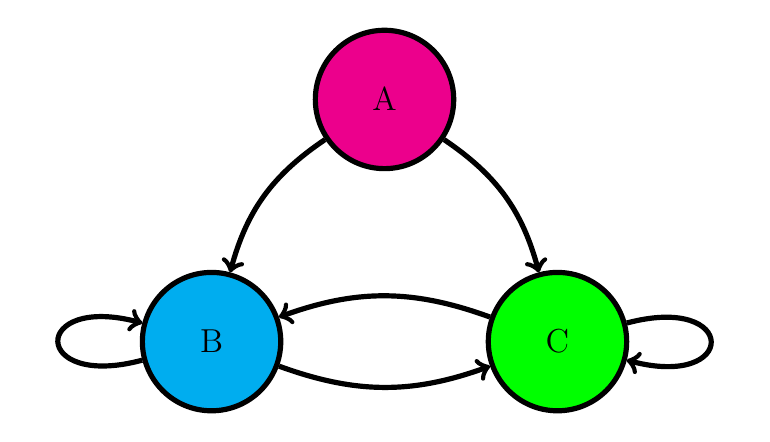
\begin{tikzpicture}
[every node/.style={inner sep=0pt}]
\node (1) [circle, minimum size=50.0pt, fill=magenta, line width=1.875pt, draw=black] at (187.5pt, -62.5pt) {\textcolor{black}{\large A}};
\node (2) [circle, minimum size=50.0pt, fill=cyan, line width=1.875pt, draw=black] at (125.0pt, -150.0pt) {\textcolor{black}{\large B}};
\node (3) [circle, minimum size=50.0pt, fill=green, line width=1.875pt, draw=black] at (250.0pt, -150.0pt) {\textcolor{black}{\large C}};
\draw [line width=1.875, ->, color=black] (1) to  [in=105, out=326] (3);
%\draw [line width=1.875, ->, color=black] (3) to  [in=285, out=146] (1);
\draw [line width=1.875, ->, color=black] (1) to  [in=75, out=214] (2);
%\draw [line width=1.875, ->, color=black] (2) to  [in=255, out=34] (1);
\draw [line width=1.875, ->, color=black] (2) to  [in=200, out=340] (3);
\draw [line width=1.875, ->, color=black] (3) to  [in=20, out=160] (2);
%\draw [line width=1.875, ->, color=black, loop above] (1) to (1);
\draw [line width=1.875, ->, color=black, loop left] (2) to (2);
\draw [line width=1.875, ->, color=black, loop right] (3) to (3);
% \node at (236.875pt, -93.125pt) [rotate=305] {\textcolor{black}{$\beta$}};
% \node at (200.625pt, -119.375pt) [rotate=306] {\textcolor{black}{Label}};
%\node at (138.125pt, -93.125pt) [rotate=55] {\textcolor{black}{\large $\alpha$}};
%\node at (174.375pt, -119.375pt) [rotate=55] {\textcolor{black}{\large $\beta$}};
%\node at (187.5pt, -173.75pt) {\textcolor{black}{\large $\gamma$}};
%\node at (187.5pt, -142.5pt) {\textcolor{black}{\large $\delta$}};
%\node at (211.875pt, -20pt) {\textcolor{black}{\large $1-\alpha$}};
%\node at (75pt, -131pt) {\textcolor{black}{\large $1-\beta - \gamma$}};
%\node at (290pt, -132.5pt) {\textcolor{black}{\large $1-\delta$}};
\end{tikzpicture}
\end{document}